\subsection*{\lr{2.1.2} فرمول‌ها به‌صورت رشته‌ای}
  همان‌طور که عبارات ریاضی را به‌صورت رشته‌هایی (توالی خطی از نمادها) می‌نویسیم، می‌توانیم فرمول‌ها را نیز به‌شکل رشته‌ای نمایش دهیم. رشته‌ی متناظر با یک فرمول از طریق \textbf{پیمایش درون‌گرد} \\ \lr{(preorder traversal)} درخت آن به‌دست می‌آید:
  \paragraph{الگوریتم \lr{2.4} (نمایش فرمول به‌صورت رشته‌ای)} \hfill \\
  \textbf{ورودی:} یک فرمول $A$ از منطق گزاره‌ای \\
  \textbf{خروجی:} نمایش رشته‌ای از $A$
  رویه‌ی بازگشتی زیر را فراخوانی کن: \lr{Inorder(A)}
  \begin{figure}[ht]
  \centering
  \begin{latin}
    \resizebox{0.55\textwidth}{!}{
    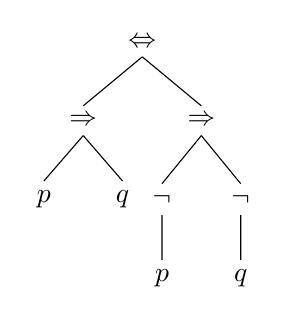
\begin{tikzpicture}[
      level distance=1cm,
      sibling distance=1.5cm,
      level 2/.style={sibling distance=1cm},
      edge from parent path={(\tikzparentnode.south) -- (\tikzchildnode.north)}
    ]
    \node {$\Leftrightarrow$}
      child { 
        node {$\Rightarrow$}
        child { node {$p$} }
        child { node {$q$} }
      }
      child { 
        node {$\Rightarrow$}
        child { node {$\neg$} child { node {$p$} } }
        child { node {$\neg$} child { node {$q$} } }
      };
    \end{tikzpicture}
    }  
  \hfill
  \resizebox{0.35\textwidth}{!}{
    \begin{tikzpicture}[
      level distance=1cm,
      sibling distance=1.5cm,
      level 2/.style={sibling distance=1cm},
      level 3/.style={sibling distance=0.7cm},
      edge from parent path={(\tikzparentnode.south) -- (\tikzchildnode.north)}
    ]
    \node {$\Rightarrow$}
      child { node {$p$} }
      child { 
        node {$\Leftrightarrow$}
        child { node {$q$} }
        child { 
          node {$\neg$}
          child { 
            node {$\Rightarrow$}
            child { node {$p$} }
            child { node {$\neg$} child { node {$q$} } }
          }
        }
      };
    \end{tikzpicture}
    }
  \end{latin}
  \renewcommand{\thefigure}{\lr{2.1}}
  \caption{دو فرمول}
  \end{figure}
  \begin{latin}
  \begin{verbatim}
  Inorder(F):
      if F is a leaf:
          print its label
          return
      Let F1 and F2 be the left and right subtrees of F
      Inorder(F1)
      print the label of the root of F
      Inorder(F2)
  \end{verbatim}
  \end{latin}
  اگر ریشه‌ی $F$ با نماد $\neg$ برچسب‌گذاری شده باشد، زیر‌درخت چپ نادیده گرفته می‌شود و مرحله‌ی \lr{Inorder(F1)} انجام نمی‌گیرد.
  \begin{definition}[تعریف \lr{2.5}]
  اصطلاح «فرمول» برای رشته نیز به‌کار می‌رود، با این فرض که به درخت زیربنایی آن اشاره دارد.
  \end{definition}
  \begin{example}[مثال \lr{2.6}]
  فرمول سمت چپ در شکل \lr{2.1} را در نظر بگیرید. پیمایش درون‌گرد این فرمول به‌صورت زیر است: ابتدا برگ سمت چپ با برچسب $p$ نوشته می‌شود، سپس ریشه‌ی آن که با $\rightarrow$ برچسب‌گذاری شده، سپس برگ سمت راست آن که $q$ است، و سپس ریشه‌ی کل درخت که با $\leftrightarrow$ برچسب‌گذاری شده، و به همین ترتیب ادامه می‌یابد. نتیجه‌ی پیمایش رشته‌ی زیر است:
  \[
  p \rightarrow q \leftrightarrow \neg p \rightarrow \neg q
  \]
  اکنون فرمول سمت راست در شکل \lr{2.1} را در نظر بگیرید. پیمایش آن نیز دقیقاً همین رشته را تولید می‌کند:
  \[
  p \rightarrow q \leftrightarrow \neg p \rightarrow \neg q
  \]
  \end{example}